\section{What is Required for Successful Optimization?}
For optimization to both succeed and be useful, several criteria must be met \citep{van2007neurofitter}:
\begin{itemize}
\item Relevance: The objective function should reflect fundamental and important properties of the data that a good model would reproduce.
\item Speed: The objective function should be fast to calculate, since typically a large number (potentially millions) of evaluations are performed during the search, many of which may require re-simulation of the model.
\item Efficient Convergence: The solution space should be as continuous and convex as possible, so that the search algorithm can rapidly converge to a global optimum.
\end{itemize}

%The EFEL signal processing suite was able to produce measurements that fulfilled the speed criteria. 

\subsection{Relevance of the Objective Function}
\subsubsection{Source of Data Constraining the Objective Function}
Due to the abundance and diversity of data available through the NeuroElectro Project \cite{tripathy2014neuroelectro}, my initial work relied heavily on that data source.
However, that data is enriched in passive membrane properties as well as the details of individual action potential waveforms.
But what distinguishes, say, a Layer 5 pyramidal cell in motor cortex from a Layer 5 pyramidal cell in visual cortex, in terms of the computational principles that systems neuroscientists might care about (e.g. decoding, information, etc.) is more likely to be reflected in the patterns of spiking and not the dynamics of single spikes or subthreshold behavior.
Furthermore, most reduced models are not implemented in way that allows for richly detailed action potential waveforms to be reproduced.

Together, this implies that reduced models optimized against data exclusively from NeuroElecto may be the worst of both worlds: they fail to capture the sub-millisecond dynamics of the action potential encoded in that data, while also failing to exhibit any of the suprathreshold dynamics (e.g. types of bursting) that distinguish one cell type from another, in the mind of a systems neuroscientist.
This problem is mitigated by including complementary data sources (like the Allen Cell Types database) that can address these dynamics.
Future optimization efforts should take care to identify the data sources that capture the dimensions of the experimental data along which meaningful differences between cell types can be resolved, and which models are rich enough to express.

\subsubsection{Number of Components in the Objective Function}
Theoretically every additional component included in the objective function--every constraint derived from some experimental feature--should make the error surface a better answer to the question, ``Is this a realistic model of the neuron of interest?".
Although they might increase the computation time required per objective function evaluation, such additional components may rapidly exclude large volumes of parameter space from unnecessary exploration.
For example, when modeling a bursting neuron, including burst-statistics as one of the features under evaluation will quickly exclude non-bursty regions of parameter space from consideration.

And yet a successful optimization recipe should not naively involve the use of all available computable features.
Some features might be biologically irrelevant, or impossible for some model class to reproduce, or have extremely discontinuous error surfaces. 
This makes the task of neuronal model optimization, much more supervised and much less automatic compared to many other machine learning paradigms --careful human guidance is needed to curate the appropriate features for the task. 

\subsection{Speed of Optimization}
\subsubsection{Speed of the Objective Function}
A large fraction of the compute cycles spent evaluating each parameter set are expended on identifying the rheobase current, thus unlocking the calculation of several subsequent measurements.
Fortunately, for slower model implementations this can be sped up significantly through parallelism, as described in section \ref{sec:parallel-rheobase}.
In some applications, parallel code scheduling is incompatible with with the just-in-time (JIT) compilation approach described in Section \ref{sec:new-models}, so parallelism sometimes trade off against raw model simulation speed. 

\subsubsection{Speed of Parallel Exploration}
In this work it was sometimes memory pressure and not clock speed that produced the major bottleneck.
This was especially true when mining features from pre-existing databases.
In these contexts I made use of a delayed iterator provided by the Dask library Dask \citep{rocklin2015dask} to stream very large amounts of data in memory-friendly chunks as needed.
Delayed evaluation using the Dask library also resolved conflicts Additionally delayed evaluation caused fewer conflicts with JIT code.
%timlyness of results was not the fundamental 
%Additionally the dask delayed algorithm
%In this context there were two different classes of model: 
%Models that should have parallel Rheobase or parallel chromosome evaluation.

%Caching of simulation results can also speed up evaluation, for example when computing multiple features based upon the same simulated membrane potential trace (e.g. spike count and time to first spike at a given current amplitude).
% Although this is an obvious opportunity for speed up, it was abandoned as the first pass attempt at solving this inside Neuronunit lead to unpredictable bugs for the whole team of programmers involved. This would probably work in current versions of neuronunit.
%XXXX More about speed here.




%\subsection{More about Rastrigin's function...?}
%Rastrigin's function has convexity in two scales. On the larger scale the surface %has a convex property, on the small scale the function is uniformly pocked with %minima wells. In order for the GA to optimize Rastrigin's function it must be %able to exploit the global information of the error surface, and simultaneously %the genes will often converge for generations in the minima, but they won't get %stuck there for two reasons: Reason 1, the global convex shape will be %represented in some genes that participate in cross over, therefore it is %learnable. Reason 2:
% mutation and cross-over provide a significant repulsive force, driving %chromosomes to test other locations despite that they perceive those locations to %be less optimal.\\
   %\begin{figure}
  %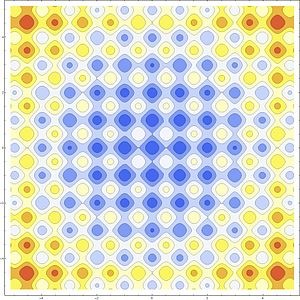
\includegraphics[]{figures/rastagrind.jpg}
  %\caption{}
   %\end{figure}
   
%   It is worth noting that although Rastrigrins function is challenging it does not the present the worst gradient to learn from. Worse than Rastrigrins function, are functions that on a large scale are flat, but on the smaller scale contain a high density ripples.
%   but lacks this global convex trend, excepting for an abrupt and localised descent to the optima.
   
%   Without some first prior knowledge of the error surface, a likely outcome is to attempt optimize on uninformative surfaces. If an uninformative surface is applied, it does not mean that the genetic algorithm will not succeed, it only means that the performance of the GA may be only marginally better than random sampling, or exhaustive search of the error surface.
   %Random sampling, sounds bad, however, if the best random solution is digitally stored, and the number of samples applied is less than the possible number of samples in an exhaustive search, random sampling may better resolve the exploitation/exploration dilemna than both gradient descent, and exhaustive search.
 

   
  
